\chapter{Theoretical and phenomenological background}
\label{ch:background}
\graphicspath{{Chapter-Background/figures/}}

\section{Quantum chromodynamics}
\subsection{History and experimental motivation}

The atomic nucleus was discovered in the early 20th century \cite{Rutherford:1911zz}, and a few years later it was determined that it was composed of protons ($p$).
An additional, electrically-neutral nuclear constituent particle was proposed soon after and the neutron ($n$) was finally discovered in the early 1930s \cite{Chadwick:1932ma}.
Clearly some new type of interaction, strong enough to overcome electrostatic repulsion between protons, bound the nucleons ($p$ and $n$) together in the nucleus.
A particle field was proposed to mediate this strong interaction, dubbed the pion ($\pi^\pm$, $\pi^0$) \cite{Yukawa:1935xg}.
Since the strong interaction only acts over a length scale of about 2 fm, the mediating pion was predicted to have a mass of about 100 \MeV\footnote{The potential mediated by a boson of mass $m$ is proportional to \( - \exp(-mcr/\hbar)/r\), where $r$ is the separation between a pair of participants. Thus the mass of a mediating boson for a potential with a characteristic cutoff length of $\lambda$ is $m = \hbar/c\lambda = \frac{200 \MeVcc \textrm{fm}}{\lambda}$.}.
The charged pion was indeed discovered experimentally in 1947 \cite{Lattes:1947mw}.
Pions can be interpreted as the Nambu-Goldstone bosons corresponding to the spontaneously broken chiral symmetry, which explains their relatively small masses.

The expanding body of observed hadrons\footnote{a particle bound by the strong nuclear interaction} and their allowed decays suggested additional conserved quantum numbers suggested that they could be composed of constituent particles.
It was noticed that hadrons can be organized by their quantum numbers in a manner described by an $SU(3)$ \emph{flavor} symmetry \cite{GellMann:1962xb}.
This suggests that hadrons are composed of constituent particles called \emph{quarks}; however, the quark model was not immediately accepted because free quarks were not (and still have not been) observed.
Because electrons are point-like particles to the limits of current experiments, a scattering process $e^- A \rightarrow e^- X$ is dependent only on the internal structure of the target $A$.
The electron scatters through a virtual photon that interacts directly with the hadron in a process called \ac{DIS}\footnote{``deep'' because it probes the constituent structure of the target, ``inelastic'' because kinetic energy and matter are exchanged in the creation of the product particles}.

\begin{figure}[t]
  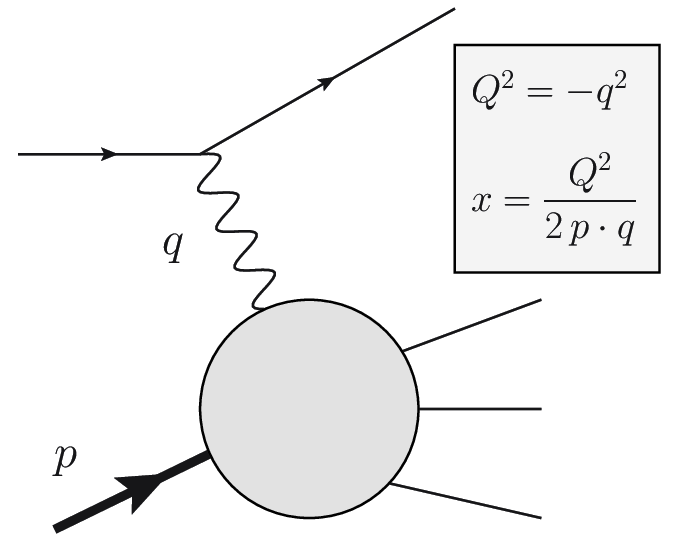
\includegraphics{dis_electron_proton.png}
  \caption{Deep inelastic scattering of a lepton on a hadron. Figure from \Ref{\cite{dis_fig_proceedings}}.
}
  \label{fig:dis}
\end{figure}

Under the constraints of Lorentz and gauge invariance, the cross-section of an unpolarized \ac{DIS} process with incoming lepton and proton momenta $k$ and $P$ respectively and momentum transfer $q$ can be expressed as \cite{Tanabashi:2018oca}
\begin{equation}
  \frac{d^2 \sigma}{dx \, dQ^2} = \frac{4\pi\alpha^2_\textrm{EM}}{2xQ^4}\left[ \left(1+(1-y)^2\right) F_2\left(x, Q^2\right) - y^2 F_L \left(x, Q^2\right) \right]
  \label{eq:dis}
\end{equation}
where $Q^2 = -q^2$ is the absolute magnitude squared of the photon's virtuality, $x = \frac{Q^2}{2q \cdot P}$, and $y = \frac{q \cdot P}{k \cdot P}$ is the fraction of the lepton's energy lost in the nucleon's rest frame.
In the parton model, which describes the proton as approximately-free point-like quarks in the infinite longitudinal momentum frame, $x$ is interpreted as the fraction of the target proton's momentum carried by a struck parton.
The structure functions $F_i(x, Q^2)$ describe the inherent internal structure of the proton.
The longitudinal structure function $F_L = F_2 - 2xF_1$ is zero by the Callan-Gross relation \cite{Callan:1969uq}, and experimentally the ratio $2xF_1 / F_2$ is consistent with 1 independent of $x$.
In the parton model, where the proton is described in terms of free point-like quarks constituents, the structure function $F_2$ is decomposed into \acp{PDF}
\begin{equation}
F_2 \left(x, Q^2\right) = x \sum_q e_q^2 f_{q/p}(x)
\end{equation}
to lowest order in the strong coupling constant $\alpha_s$.
The independence of $Q^2$ of the \acp{PDF} is a manifestation of their point-like description in the parton model and is known as \emph{Bjorken scaling}.
Logarithmic corrections are understood theoretically and arise as gluon radiation from the quarks becomes relevant, particularly at small $x$ (\Cref{fig:proton_f2}).

\begin{figure}[t]
  %% page 326 of particle review
  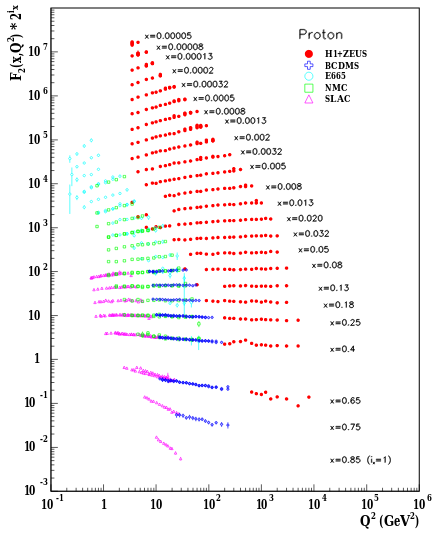
\includegraphics[width=0.45\linewidth]{proton_f2.png}
  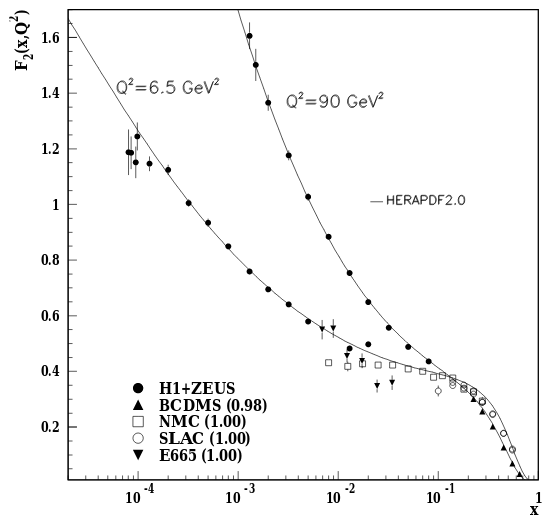
\includegraphics[width=0.54\linewidth]{proton_f2_vs_x.png}
  \caption{The structure function $F_2\left(x, Q^2\right)$ of the proton as a function of $Q^2$ (left) and of $x$ (right). Figure from \Ref{\cite{Tanabashi:2018oca}}.}
  \label{fig:proton_f2}
\end{figure}

%% TODO: could discuss R_had as evidence for spin-1/2 quarks ??

An experimental and phenomenological description of the nucleon structure functions does not provide a complete description of the interactions among nucleon constituents.
The success of gauge theories in describing \ac{QED} ($U(1)$) and electroweak theory ($U(2) = SU(2) \otimes U(1)$) suggests that some other gauge theory may be able to describe the nuclear interaction.
A quantum field theory with an $SU(N_c)$ ``color'' symmetry with $N_c$ colors, called \qcd, is one such candidate.
For it to be a believable description of the strong interaction, it must not only be consistent with experimental observations, but it must also explain why free quarks have never been observed.
The rate of hadronic production in electron-positron collisions is proportional to $N_c$, so experimental measurements of the ratio\footnote{at energies above the $b\bar{b}$ threshold and below the mass of the $Z$ boson}
\begin{equation}
R \equiv \frac{\sigma\left(e^+ e^- \rightarrow \textrm{hadrons}\right)}{\sigma\left(e^+ e^- \rightarrow \mu^+ \mu^- \right)} \approx N_c \sum_{q \in \{u,d,s,c,b\}} e_q^2 = \frac{11}{9} N_c
\end{equation}
have been made to determine the number of colors, showing very good agreement with a value of $N_c = 3$.
Though the non-abelian character of \qcd makes many practical calculations difficult, it has shown remarkable success in describing the strong interaction, as will be discussed in the remainder of this section.

\subsection{The QCD Lagrangian}
The gauge-invariant lagrangian density of \qcd \cite{Wilczek:2000ih} is that of an $N_c=3$ Yang-Mills theory given by
\begin{equation}
  \Lagr_\mathrm{QCD} \equiv -\frac{1}{4} G^a_{\mu\nu}G^{a\mu\nu} + \bar{\psi} \left( i \slashed{D} - m \right) \psi \; .
\end{equation}
Here repeated indices are summed, where $\mu$ and $\nu$ indicate spacetime indices, $a$, $b$, and $c$ indicate color indices in the fundamental ($N=3$) representation, and $A$, $B$, and $C$ indicated color indices in the adjoint ($N=8$) representation.
The slash notation refers to contraction with the gamma matrices $\{\gamma^\mu, \gamma^\nu\} = 2\eta^{\mu\nu}$\footnote{with Minkowski signature $(+---)$}.
The covariant derivative
\[ D_\mu \equiv \partial_\mu - i g A^C_\mu t^C\]
where $A^C_\mu$ is the gluon field, $t^C$ are the generators of the $SU(3)$ gauge group, and $g$ is the strong charge constant.
The constant $g$ in the lagrangian is always squared when computing rates from quantum amplitudes, so physical results are typically expressed in terms of
\begin{equation}
  \alpha_s \equiv \frac{g^2}{4\pi} \; ,
\end{equation}
typically called the strong coupling constant.
The gluon field strength tensor is
\[ G^A_{\mu\nu} \equiv \partial_\mu A^A_\nu - \partial_\nu A^A_\mu + g f^{ABC} A^B_\mu A^C_\nu \]
with the $SU(3)$ structure constants defined such that
\[ [t^A,t^B] = if^{ABC}t^C \; \footnote{In the $SU(2)$ gauge group the adjoint representation is three-dimensional and the structure constants are given by the anti-symmetric Levi-Civita symbol $\epsilon^{ABC}$}.\]
The quark fields are defined such that the mass matrix $m$ is diagonal:
\[ \bar{\psi}m\psi = \sum_{q = u,d,s,\ldots} m_{q}\bar{q}q \]
The quark masses $m_q$ are generated by the mechanism of spontaneous electro-weak symmetry breaking in which the Higgs field, coupling to fermions and electro-weak gauge bosons, acquires a nonzero vacuum expectation value.
This procedure induces in the \qcd vacuum a breaking of the chiral symmetry $SU(N_f) \times SU(N_f) \rarrow SU(N_f)$ in the massless Lagrangian.

\begin{figure}[t]
  %% page 155 of particle review
  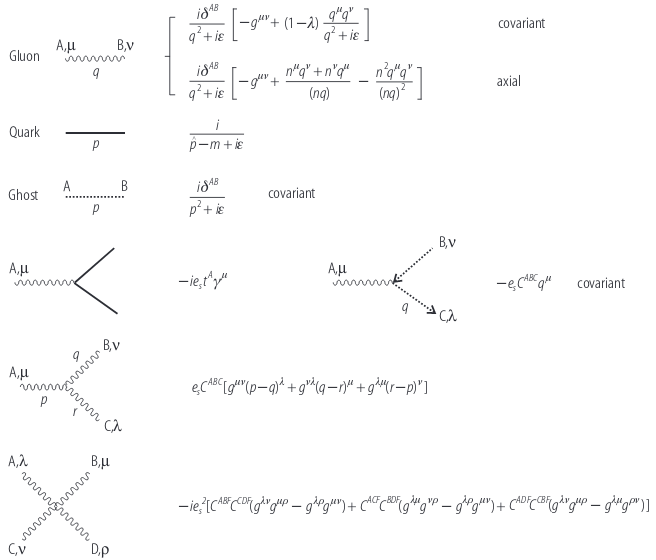
\includegraphics{qcd_feynman.png}
  \caption{The propagators and vertices in \qcd along with the corresponding Feynman rules for the amplitude factors. The strong coupling charge is written here as $e_s = \sqrt{4\pi\alpha_s}$, and the gauge parameter is denoted by $\lambda$. Figure from \Ref{\cite{Altarelli:2013tya}}.}
  \label{fig:qcd_feynman}
\end{figure}

%% The QCD Lagrangian has a symmetry under the gauge transformation defined as... %% we don't really need to get explicit about gauge transformations
The physical interaction vertices of \qcd are a 3-point quark-gluon vertex analogous to he \ac{QED} vertex, a 3-gluon vertex and a 4-gluon vertex (\Cref{fig:qcd_feynman}).
A scalar ghost field\footnote{which has a spin of 0 yet anti-commutes like a fermion} also couples to the gluon as is generally necessary in non-abelian gauge theories to prevent over-counting gauge-equivalent states \cite{Faddeev:1967fc}.
The non-abelian nature of \qcd manifests in Feynman diagrams as the gluon self-interaction vertices.
The gluon-gluon interactions make \qcd difficult to calculate with.
In a classical theory, they prevent the principle of superposition from being applied in chromodynamics.
The highly-nontrivial gluon self-interaction is a crucial ingredient in the richness of nuclear physics.


\subsection{Running of the coupling constant} %% maybe doesn't deserve its own section, instead split into UV and IR?

%% https://arxiv.org/pdf/1604.08082.pdf

As is the case in all quantum field theories, the naive calculation of higher-order (in $\alpha_s$) loop diagram integrals contain divergences in the amplitudes.
In many theories, including \qcd \cite{Gross:1973ju}, these infinities can be dealt with with a process called \emph{renormalization}.
One description of renormalization is the introduction of an energy/momentum cutoff scale.
Physical calculations cannot depend on any such scales, so amplitude calculations must be organized such that any dependence on the renormalization scale cancels in a physical result, which can be done order-by-order in perturbation theory.
This process induces a scale-dependence of the coupling constant $\alpha_s$ on the arbitrary renormalization scale $\mu$.
If the value of $\alpha_s$ is known at a particular $\mu = \mu_0$, its dependence on the scale can be determined by calculating the beta function
\begin{equation}
  \beta(\alpha_s) \equiv  \frac{\partial \alpha_s}{\partial \ln \mu^2}
\end{equation}
which to one loop is given by \cite{Gross:1973id}
\begin{equation}
  \beta(\alpha_s) = -b_0 \alpha_s^2 + \bigo{\alpha_s^3}
\end{equation}
where
\[
%% \beta_1 = \frac{11 N_c - 2 N_f}{3}
b_0 = \frac{11 N_c - 2 N_f}{12\pi}
\]
for $N_c$ colors and $N_f$ relevant quark flavors at the scale of the process.
The \ac{LO} solution is
\begin{equation}
  \alpha_s(\mu^2) = \frac{1}{b_0 \ln\left(\mu^2 / \lqcd^2\right)}
  \label{eq:running_as}
\end{equation}
where \lqcd is defined by a given value for $\alpha_s$ at a scale $\mu_0$
\[
\lqcd = \mu_0 \exp \left( -\frac{1}{2 b_0 \alpha_s(\mu_0^2)} \right) \; .
\]
The above expression for \lqcd changes depending on the order of the perturbative expansion and the renormalization scheme, but the physical meaning of \lqcd is still apparent.
It is the energy scale below which the strong coupling diverges, showing an explicit breakdown of perturbation theory.
It is noteworthy that \qcd predicts the emergence of such a scale, even in the conformal\footnote{i.e. a scale-invariant lagrangian with massless quarks} theory.
Practically the \qcd scale is often quoted around a value of %% at the 5-quark level, where \mu ~ m_Z
\[
\lqcd \approx 200 \MeV \;,
\]
but the precise value can differ by a factor of 2 or more depending on arbitrary choices such as scheme, order, and gauge.

A convenient choice for the renormalization scale $\mu$ in \Cref{eq:running_as} is to set $\mu^2 = Q^2$ for a physical process with momentum transfer $Q$.
This choice introduces some theoretical and computational wrinkles but gives a simple and direct relationship to experimental data.
Experimental values of the strong coupling constant are typically reported at the mass of the $Z$ boson, with a current world average value of
\[
\alpha_s(m_Z^2) = 0.1181 \pm 0.0011
\]
where $m_Z = 91.187 \GeV$.
The running of the coupling is demonstrated by the summary of experimental measurements in \Cref{fig:running_coupling}.

\begin{figure}[t]
  %% page 155 of particle review
  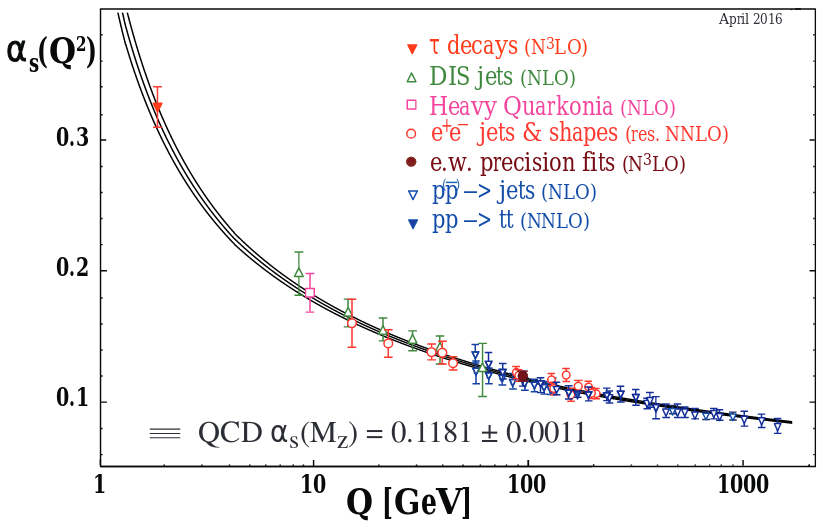
\includegraphics{running_as.png}
  \caption{Measurements of the strong coupling constant $\alpha_s$ as a function of the energy scale $Q$. Figure from \Ref{\cite{Tanabashi:2018oca}}.}
  \label{fig:running_coupling}
\end{figure}

\subsection{Asymptotic freedom}

The strong coupling constant decreases with rising energy as shown in \Cref{eq:running_as} and \Cref{fig:running_coupling}.
This phenomenon is known as \emph{asymptotic freedom} and is necessary to explain Bjorken scaling, since without this feature the interaction between quarks bound in a hadron could not be approximately ignored in a \ac{DIS} process.
It requires $b_0 > 0$, which for $N_c = 3$ \qcd is true so long as there is no scale at which additional quark fields become relevant such that $N_f > 16$.
Physically this is understood as arising from the fact that the contributions to $\alpha_s$ from gluon loops dominate those from quark loops \cite{Wilczek:2005az}.

Asymptotic freedom is not present in abelian gauge theories like \ac{QED}, where the screening of a bare electric charge causes the effective charge to decrease at large distances, or equivalently the effective electric charge increases at higher energy.
In \qcd the color field reinforces itself to induce an even stronger field, so the effective field strength does not decrease with increasing separation.

The phenomenology of jets relies heavily on asymptotic freedom.
In high energy hadronic and nuclear collisions, partons from each participant nucleon scatter with large momentum transfer.
Because the effective $\alpha_s$ is small, the product quarks and gluons are ejected with large transverse momentum and are not strongly coupled to other partons in the collision.
The stronger coupling at low $Q^2$ also means that the \qcd radiation is emitted at small relative momentum from the hard parton.
Thus the decay products of these high-energy partons are produced in a \emph{parton shower} and generate clumps of final-state particles known as jets.

\subsection{Color confinement}

In order to be trusted as a fundamental theory of nuclear interactions, \qcd must provide an understanding of the lack of experimental observation of free quarks or gluons.
Indeed the infrared divergence of $\alpha_s(Q^2)$ suggests that there is some nontrivial behavior as the separation between two colored particles is increased.
Predictions from \qcd in this region cannot be investigated using perturbation theory, since the rapidly rising coupling constant precludes the convergence of any diagram expansion.
The numerical approach of \emph{lattice gauge theory} \cite{Aoki:2016frl} is successful at reproducing a number of experimental measurements such as the light hadron mass spectrum \cite{Durr:2008zz}.
Lattice gauge theory introduces a discrete grid spacing $a$ along both spatial and temporal dimensions, which acts as a regularization parameter.
An extrapolation of vanish grid spacing $a \rightarrow 0$ is performed in order to recover the continuous theory of \qcd.

\begin{figure}[t]
  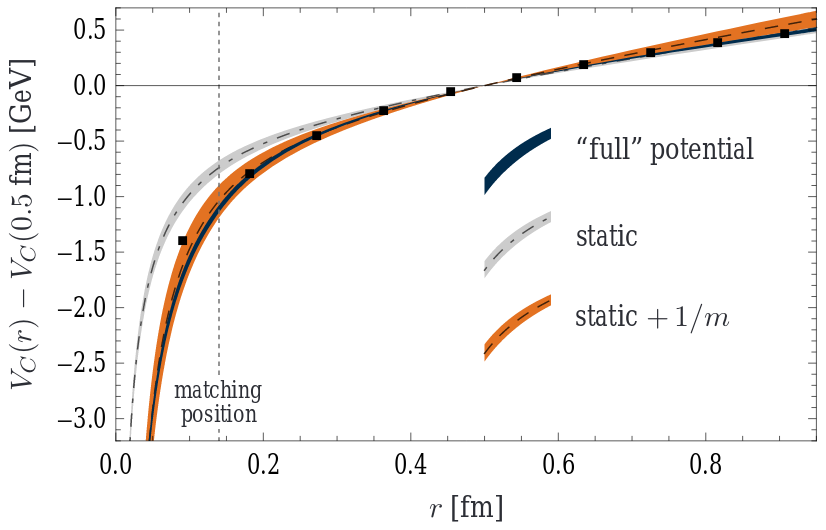
\includegraphics{ccbar_potential.png}
  \caption{Charmonium ($c\bar{c}$) potential from a combination of perturbative \qcd (small $r$) and lattice \qcd (large $r$). Figure from \Ref{\cite{Laschka:2011zr}}.}
  \label{fig:charmonium_potential}
\end{figure}

The heavy quark-antiquark potential can be computed on the lattice, as shown in \Cref{fig:charmonium_potential}.
The charmonium lattice QCD potential with three light quarks and charm-quark mass effects is well-described to the 4-loop level by the parameterization \cite{Laschka:2011zr}
\begin{equation}
V_{c\bar{c}}(r) = - \frac{A}{r} + \sigma r
\end{equation}
with $A = 160 \pm 4 \MeV\,\fm$ and $\sigma = 790 \pm 30 \MeV/\fm$ (\Cref{fig:charmonium_potential}).
The first term has the same form as an attractive Coulomb potential, albeit with a coupling constant about 2 orders of magnitude larger than the \ac{EM} coupling\footnote{where $\alpha_\textrm{EM} \hbar c \approx 1.44 \MeV\,\fm$}.
The latter term resembles the potential from the force by a string of constant tension $\sigma$, which invokes a description by color ``flux tubes'' between the two quarks of constant energy per length.
This ``string'' term increases without bound at large separations, so a quark-antiquark pair cannot be separated with a finite amount of energy.
At some point it becomes more energetically favorable to produce a quark-antiquark pair out of the vacuum than to maintain a long flux tube (\Cref{fig:qqbar_flux}).
This property is responsible for the phenomenon of \emph{confinement}, which is the absence in nature of bare color charges.

\begin{figure}[t]
  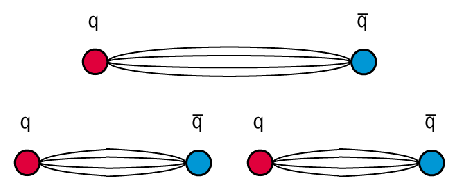
\includegraphics{qqbar_flux.png}
  \caption{The color flux tube between a quark-antiquark pair and the breaking of the flux tube into a new $q\bar{q}$ pair from the vacuum.}
  \label{fig:qqbar_flux}
\end{figure}


\section{QCD at high temperatures}

Given the observed properties of asymptotic freedom and color confinement, a natural question is whether nuclear matter has a phase transition at large density and/or temperature.
In a system with a low number of quarks, the color connection keeps each bound tightly to others.
At high densities, however, individual flux tubes are not discernible, and individual color charges are easily balanced by nearby color sources.
Such a state could exhibit deconfinement, with color charge free to move as electric charge does in a conventional plasma.
This \qgp is expected to have different properties than hadronic matter.

\begin{figure}[t]
  %% https://homepages.uni-regensburg.de/~sow28704/ftd_lqcd_ss2012/ftd_lqcd_ss2012.html
  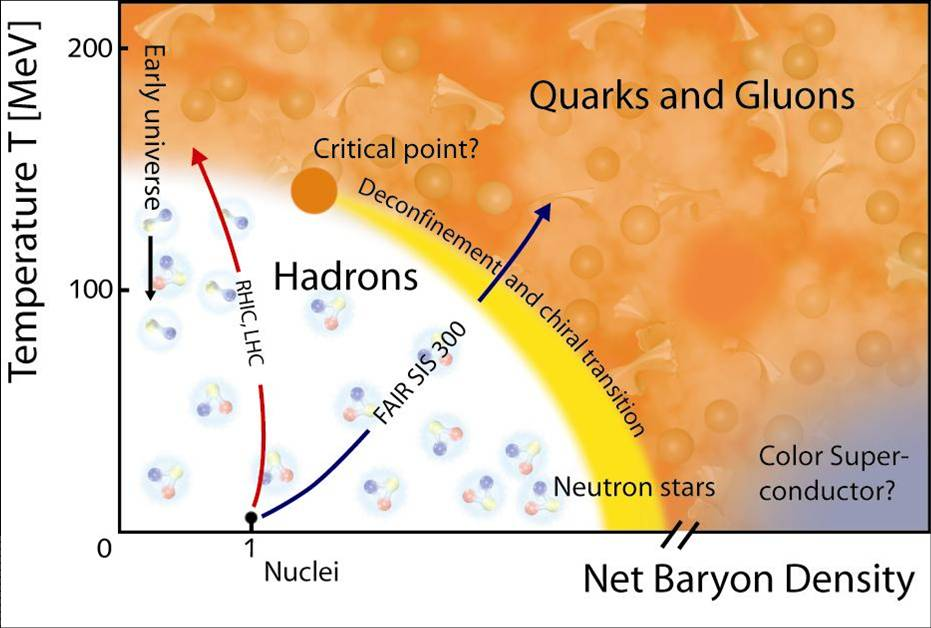
\includegraphics{qcd_phase.jpg}
  \caption{A conjectured phase diagram for QCD matter. The transition from hadronic matter to QGP at low baryon density is a smooth crossover. A critical point is hypothesized but not established.}
  \label{fig:qcd_phase}
\end{figure}

Dimensional analysis suggests that the critical temperature $T_c$ (at zero chemical potential) should be close to the only possibly relevant scale
\[
T_c \sim \lqcd \sim 10^{12}~\mathrm{K}\; .
\]
\Cref{fig:qcd_phase} shows a conjectured phase diagram for \qcd matter.
The transition between hadronic matter and the QGP is a smooth crossover at low baryon density \cite{Aoki:2006we}.
Above some critical baryon density the transition is hypothesized to be first-order based on a number of model approaches, but this has not been established.

\subsection{Equation of state from lattice calculations}

%% the latter HotQCD ref is slightly more recent and has many good plots including static potential (no 1/m corrections?)
Thermodynamic quantities can be computed in lattice \qcd at small chemical potential \cite{Borsanyi:2013bia,Bazavov:2014pvz}.
The results are clearly distinct from the \ac{HRG} model \cite{Huovinen:2009yb}, indicating that deconfinement is a fundamental property of the transition.
The trace anomaly $T_\mu^\mu = \varepsilon - 3 p$, where $\varepsilon$ is the energy density and $p$ is the pressure, is computed in lattice calculations as a function of temperature.
It vanishes in a conformal theory, so the appearance of a significant trace anomaly with a peak around $200 \MeV$ suggests the emergence of a scale-dependence.
The pressure is related to the derivative of the trace anomaly up to factors of the temperature.
From there, the remaining combinations of thermodynamic quantities such as $\varepsilon(T)$ and the entropy density $s = \frac{\varepsilon + p}{T}$ are determined  (\Cref{fig:lattice_eos}).
A smooth crossover is observed, with a critical temperature of \( T_c = 170 \pm 4 \MeV \) \cite{Aoki:2009sc}, which is indeed close to \lqcd as predicted by dimensional analysis.
Above the critical temperature, clear deviations are shown from the predictions of the \ac{HRG} model.

\begin{figure}[t]
  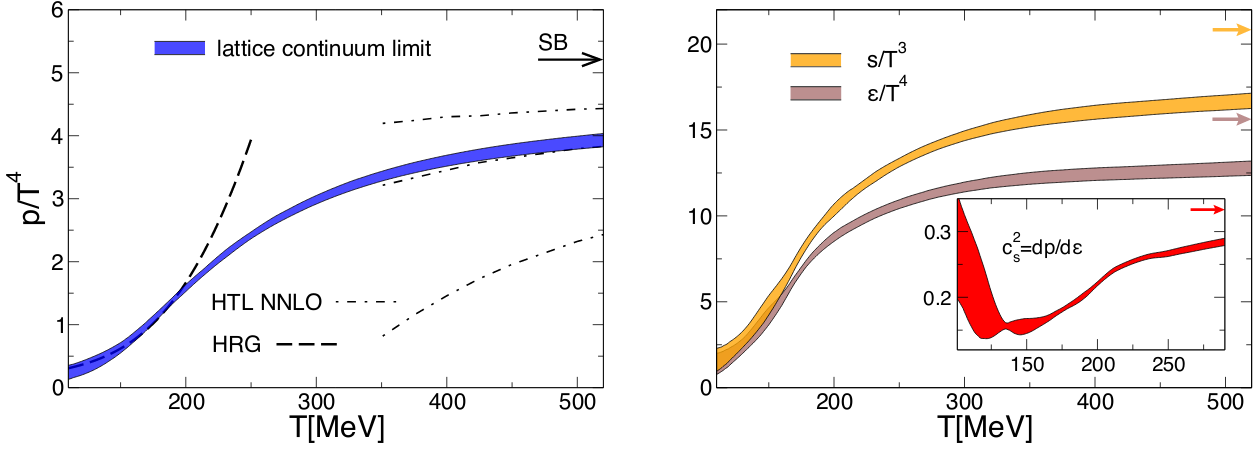
\includegraphics[width=\linewidth]{lattice_eos.png}
  \caption{The trace anomaly for several values of lattice spacing $N_\tau = 1/aT$ and the continuum extrapolation (left), and thermodynamic quantities in the continuum limit (right), both shown as a function of temperature. The solid lines show the predictions from the HRG model, and the Stefan-Boltzmann limit at $95\pi^2/60$ is shown by the straight dashed line. Figure from \Ref{\cite{Bazavov:2014pvz}}.}
  \label{fig:lattice_eos}
\end{figure}

%% The Stefan-Boltzmann limit of \(\varepsilon = \frac{g \pi^2 T^4}{30}\) where g is a degeneracy factor is not reached in lattice calculations.

\subsection{Experimental evidence for the existence of the QGP}
glauber model: this shouldn't go here per se: \cite{Miller:2007ri} %%  glauber model in HI. where does this go?
separate section on HI collisions? with p+Pb maybe not so necessary


\section{Hydrodynamic description of heavy ion collisions}

\subsection{Relativistic fluid dynamics}

%% Poincar\'e instead of Lorentz?
Under the constraints of Lorentz symmetry and neglecting fluctuations, the stress-energy tensor of a perfect fluid described by flow four-velocity $u^\mu(x^\nu)$ is
\begin{equation}
%% T^{\mu\nu} = \left( \varepsilon + p \right) u^\mu u^\nu - p g^{\mu\nu} %% metric term has opposite sign for time-positive metric
T^{\mu\nu}_{(0)} = \varepsilon u^\mu u^\nu + p \Delta^{\mu\nu}
\end{equation}
where $\varepsilon$ and $p(\varepsilon)$ are respectively the energy density and pressure in the local rest frame and \( \Delta^{\mu\nu} \equiv -g^{\mu\nu} + u^\mu u^\nu \) is the space-like projection operator\footnote{The four-velocity $u^\mu$ is itself the time-like projection operator.}.
In the absence of sources there are four conserved quantities corresponding to energy and three components of momentum.
\begin{equation}
  \label{eq:em_cons}
  \nabla_\mu T^{\mu\nu} = 0
\end{equation}
Projecting this equation into time and space components yields the relativistic Euler equations
\begin{align}
  D\varepsilon + \left(\varepsilon + p\right)\nabla^\perp_\mu u^\mu &= 0 \\
  \left(\varepsilon + p\right)Du^\mu + c_s^2 \nabla_\perp^\mu \varepsilon &= 0 
\end{align}
where \(D \equiv u^\mu \nabla_\mu\) is the co-moving time-like derivative, \( \nabla_\perp^\mu \equiv \Delta^{\mu\nu} \nabla_\nu \) is the co-moving space-like derivative, and \(c_s(\varepsilon) \equiv \sqrt{\frac{\partial p}{\partial \varepsilon}} \) can be identified with the speed of sound.

The assumption of perfect fluidity can be relaxed by adding the terms
\begin{equation}
T^{\mu\nu} = T^{\mu\nu}_{(0)} + \pi^{\mu\nu} + \Delta^{\mu\nu}\Pi
\end{equation}
where $\pi^{\mu\nu}$ and $\Pi$ are the shear stress and bulk stress and split the corrections into a traceless and trace part respectively.
To first order in gradients of $u^\mu$ and $\varepsilon$,
\begin{align}
  \label{eq:shear_stress}
  \pi^{\mu\nu} &= - \eta \sigma^{\mu\nu} \\
  \label{eq:bulk_stress}
  \Pi          &= - \zeta \nabla^\perp_\mu u^\mu
\end{align}
with
\begin{equation}
  \label{eq:sigma_tensor}
  \sigma^{\mu\nu} \equiv \nabla_\perp^\mu u^\nu + \nabla_\perp^\nu u^\mu - \frac{2}{3} \Delta^{\mu\nu}\nabla^\perp_\alpha u^\alpha \; ,
\end{equation}
and $\eta$ and $\zeta$ are the first order \emph{transport coefficients} and are called respectively the shear viscosity and bulk viscosity.
Applying energy-momentum conservation (\Cref{eq:em_cons}) with these 1st-order corrections yields the relativistic Navier-Stokes equations, but these equations violate causality by instantaneously propagating gradients to viscous stresses.
This causes instabilities in the solutions to these equations.
Causality can be recovered by expanding to second-order in the gradients \cite{Israel:1976tn} at the cost of introducing 15 second-order transport coefficients, four of which vanish in flat spacetime.
State-of-the-art simulations of the \qgp rely on second-order relativistic hydrodynamics \cite{Israel:1979wp}.

\subsection{Applicability of hydrodynamics}
%% low viscosity: large cross-section, low mfp

In order for hydrodynamics to be capable of a valid description, additional terms in the expansion of $T^{\mu\nu}$ must be small compared to existing terms.
The magnitude of the $\sigma^{\mu\nu}$ gradients in \Cref{eq:sigma_tensor} can be estimated by the inverse system size $L^{-1}$.
The 1st-order term must be small compared to the 0th-order term, so a condition for the validity of hydrodynamics is %% eta/(ep+p) from arxiv:1712.05815 \cite{Romatschke:2017ejr} pg. 28
\begin{equation}
  \frac{\eta}{(\varepsilon + p)L} \ll 1 \;.
\end{equation}
With the approximation that the mean free path is \(\lambda_\textrm{mfp} = \frac{\eta}{\varepsilon + p} \), the condition is expressed in terms of the Knudsen number
\begin{equation}
  \mathrm{Kn} \equiv \frac{\lambda_\textrm{mfp}}{L} \ll 1 \;.
\end{equation}

The series produced in the hydrodynamic gradient expansion is not convergent \cite{Denicol:2016bjh}.
This is because the number of terms grows like the factorial of the order of the expansion, and there is no lucky magic that exponentially suppresses the magnitude of the transport coefficients.
The Knudsen number in heavy ion simulations is not typically orders of magnitudes below unity \cite{Niemi:2014wta}; however, low-order viscous hydrodynamics has had ``unreasonable success'' at describing many global properties of heavy ion collisions.

Recent work has shown that the hydrodynamic expansion can be Borel-resummed \cite{Romatschke:2016hle,Romatschke:2017vte}, a method that produces an analytic continuation of the series.
The stress-energy tensor is split into a hydrodynamic attractor and a non-hydrodynamic component, with the cost that the transport coefficients become explicit functions of $\varepsilon$ and the gradients of $\varepsilon$ and $u^\mu$.
The condition for the applicability of hydrodynamics is weakened to the statement that the non-hydro modes are negligible.
It appears in many examples that the non-hydro modes decrease exponentially quickly, which potentially explains the ``unreasonable success'' of viscous hydrodynamics.
This also helps to explain the observations of some hydro-like phenomena in \pPb and even \pp collisions, where the small system size results in Knudsen numbers that are often greater than unity.


\subsection{Viscosity of the QGP and the AdS/CFT correspondence}

first discuss calculation of transport coefficients from ``first principles'', possibly show result from kinetic theory?
gylassy: 1985 eta/s \cite{Danielewicz:1984ww} %% from uncertainty principle

One of the most influential theoretical developments of the past few decades is the conjectured relationship between quantum gravity in an \ac{AdS} space and a strongly-coupled \ac{CFT} \cite{Maldacena:1997re}.
This so-called \emph{\ac{AdS}/\ac{CFT} correspondence} allows calculations in a non-perturbative \ac{CFT} to be replaced by an associated calculation in weakly-coupled gravity.

eta/s from ADS/CFT \cite{Kovtun:2004de}

%% \subsection{Fourier decomposition of particle production}
\subsection{Success of hydrodynamics}
\subsection{Flow in small systems}
 review of small-systems hydro: \cite{Nagle:2018nvi}

%% \section{Jet production and fragmentation} %% not the higher priority for us
%% Though the focus of this thesis is not on the physics of jet fragmentation, control of hard processes is essential to correctly extract observable quantities of interest.
%% This section will describe the physics behind jets.
%% TODO: Some of this discussion may be better moved elsewhere; for instance, nuclear modification may be appropriate in ``evidence for QGP''
%% \subsection{Parton model}
%% lorentz contraction in infinite momentum frame, transverse freeze-out, factorization
%% \subsection{Fragmentation function}
%% \subsection{Nuclear modification}


\section{Femtoscopy in heavy ion collisions}
This section will describe from a theoretical perspective what femtoscopy is and what it aims to achieve. The application of these techniques to experimental data will be addressed in \Cref{ch:analysis}.
\subsection{Imaging the source density function}
\subsection{Parameterization of the correlation function}
\subsection{Final-state interactions}
justify ignoring strong force; describe Coulomb correction (save jet fragmentation details for later)
\subsection{Motivation for femtoscopy in proton-lead}
\subsubsection{Collective expansion}

%% HI summary plots: (v2, RAA, etc)
%% https://atlas.web.cern.ch/Atlas/GROUPS/PHYSICS/CombinedSummaryPlots/HION/
